\documentclass[xcolor=svgnames]{beamer}
\usepackage{multirow,textcomp,color}
\usepackage{rotating}
\usepackage{amssymb,amsfonts,amsmath}
\usepackage{mathptmx,bm}
\usepackage{epsfig}
\usepackage{natbib}
\usepackage{graphicx}

% Find colour names http://calque.pagesperso-orange.fr/latex/latexps.html
%[xcolor=dvipsnames]

\usecolortheme[named=DarkBlue]{structure} % colour from svgnames
%\usecolortheme[named=Gray]{structure} % colour from svgnames
%\usecolortheme[named=LightGray]{structure} % colour from svgnames
%\usecolortheme[named=LightBlue]{structure} % colour from svgnames
%\usecolortheme[named=Teal]{structure} % colour from svgnames
%\usecolortheme[named=OliveGreen]{structure} % colour from dvipsnames
%\usefonttheme{serif}
%\usetheme{Rochester}
\usetheme{Singapore}
\setbeamertemplate{footline}[frame number]
%\setbeamercolor{frametitle}{fg=DarkBlue,bg=Tan}
%\setbeamercolor{title}{fg=DarkRed,bg=LightGray}
%\setbeamercolor{title}{fg=Navy,bg=Wheat}
\setbeamerfont{frametitle}{size=\Large,series=\bfseries}
\setbeamerfont{title}{size=\Large,series=\bfseries}

\begin{document}
%%%%%%%%%%%%%%%%%%%%%%%%%%%%%%%%%%%%%%%%%%%%%%%%%%%%%%%%%%%%%%%%%%%%%%%%%%%%%
\title{Cluster prediction by statistical modeling for Ordinal Data}
\author{Quan Zhao ({\tt felixz2010@gmail.com})\\[1em]
{\em student id: 300471028}\\[1em]
}

\date{16 Feb 2024}

%-----------------------------------------------------------------------------

\begin{frame}\frametitle{
}
\titlepage
\end{frame}

%-----------------------------------------------------------------------------

\begin{frame}\frametitle{Outline}

\begin{enumerate}
\item Introduction
\begin{itemize}
\item Ordinal data
\item Clustering
\item Finite Mixture Models
\end{itemize}
\item Methods
\item Research Goals
\end{enumerate}

\end{frame}
%-----------------------------------------------------------------------------

\begin{frame}\frametitle{Ordinal data}

% {\bf The response variable has ordinal categorical scales}

Ordinal data, a pivotal concept in statistical analysis, represents categorical data characterized by a meaningful order among its categories, without implying uniform differences between these ranks.

% \begin{minipage}
%   {0.6\textwidth}{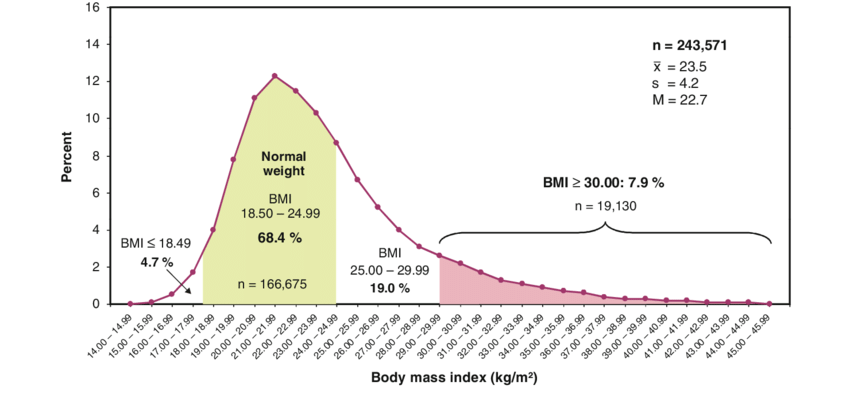
\epsfig{file=images/bmi_2,width=1.3\linewidth}}
%   ~\cite[]{aaron2023explain}
% \end{minipage}

\begin{figure}
  \centering
  % If you continue using \epsfig
  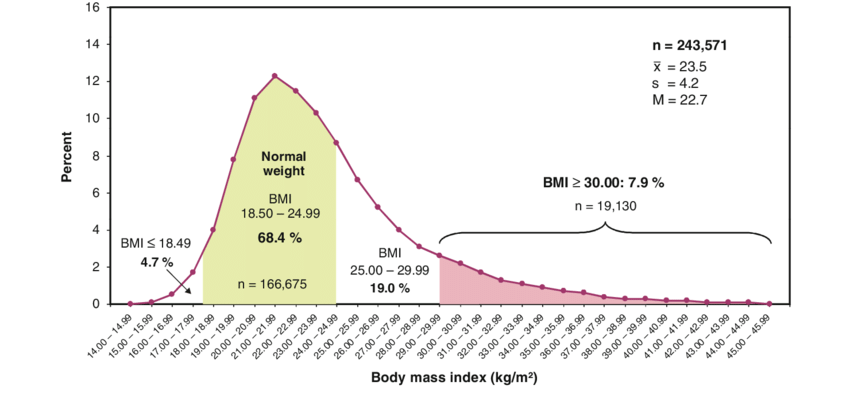
\epsfig{file=images/bmi_2,width=0.6\linewidth}
  % If you switch to \includegraphics from the graphicx package
  % 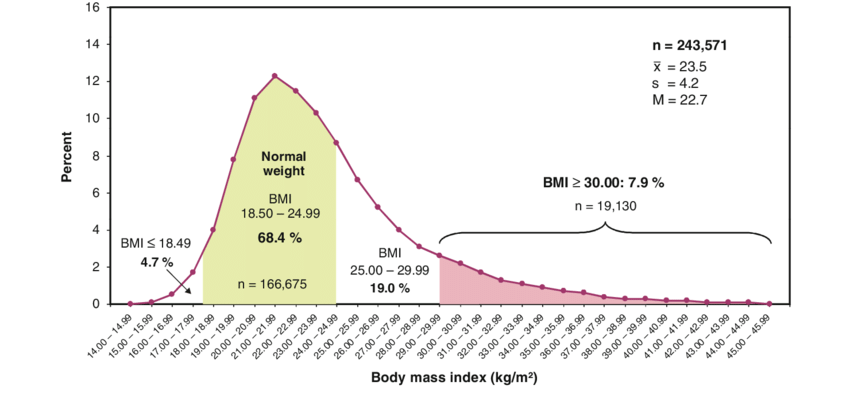
\includegraphics[width=0.6\linewidth]{images/bmi_2}
  \caption{BMI Categories~\cite{article}}
\end{figure}


% \begin{itemize}
% \pause
% \item  \textcolor{blue}{Likert scale}:  ``strongly disagree'', ``disagree'', ``agree'', or ``strongly agree'' in a survey.
% \pause
% \item \textcolor{blue}{Braun-Blanquet cover-abundance scale} is very common in vegetation analysis. 
% \end{itemize}

\end{frame}


%-----------------------------------------------------------------------------
\begin{frame}\frametitle{Clustering}

  Distance based clustering approach relies on the concept of similarity or distance between data points. The aim is to minimize the distance between data points within a cluster while maximizing the distance between data points in different clusters. Popular methods include K-means, hierarchical clustering, and DBSCAN, each using different metrics (e.g., Euclidean, Manhattan) to measure distance or similarity

  \begin{figure}
    \centering
    % If you continue using \epsfig
    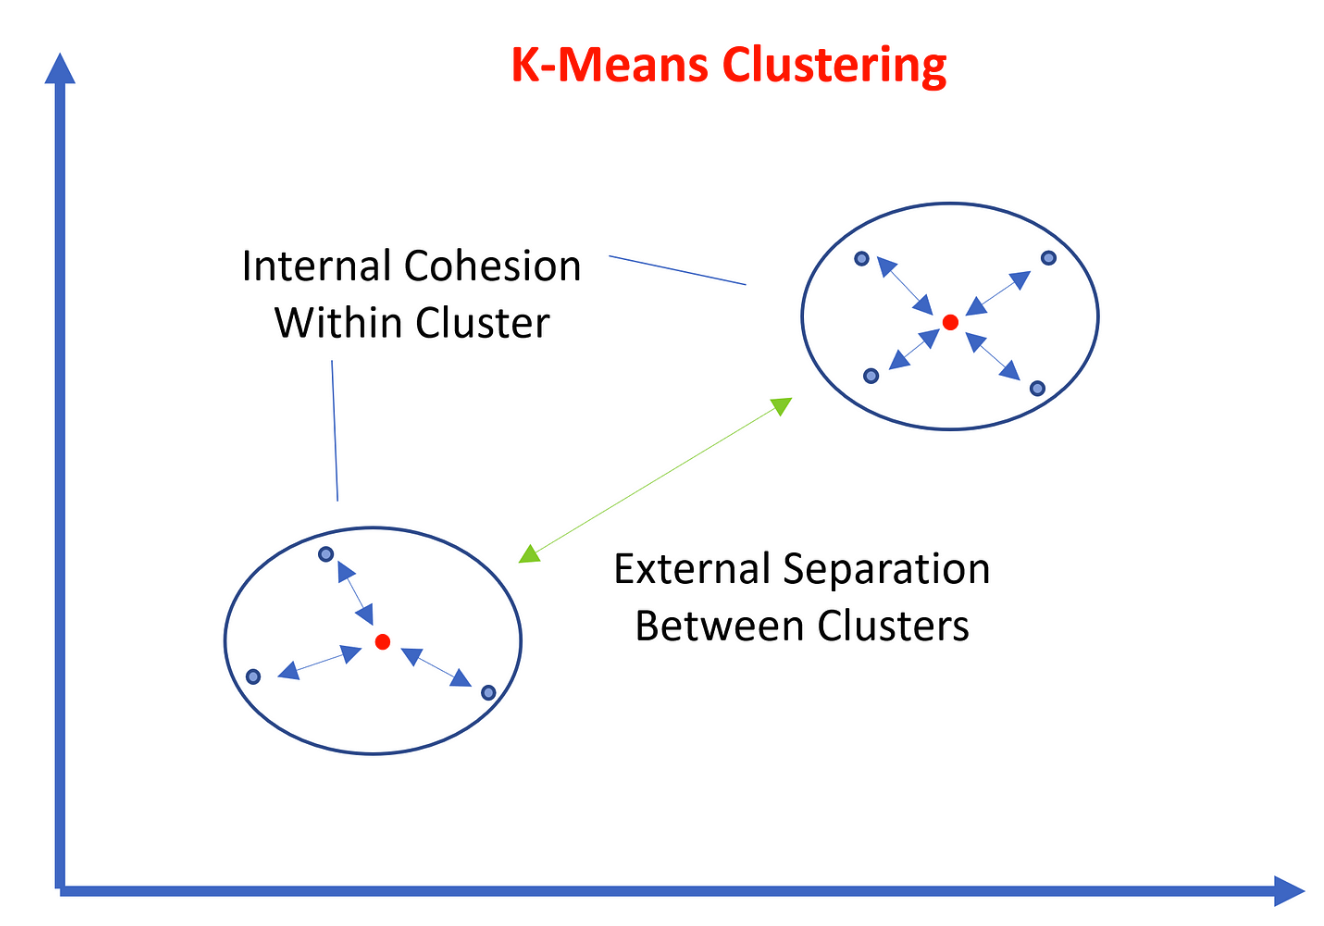
\epsfig{file=images/clustering_2,width=0.48\linewidth}
    % If you switch to \includegraphics from the graphicx package
    % 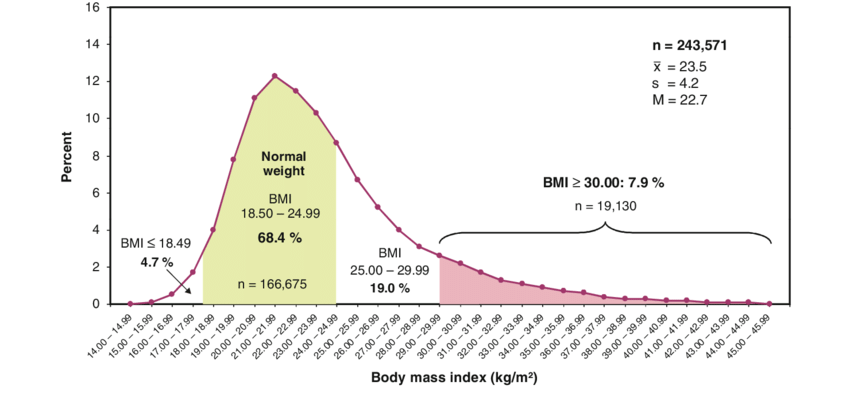
\includegraphics[width=0.6\linewidth]{images/bmi_2}
    \caption{Distance based Clustering~\cite{aaron2023explain}}
  \end{figure}

  % \begin{minipage}
  %   {0.5\textwidth}{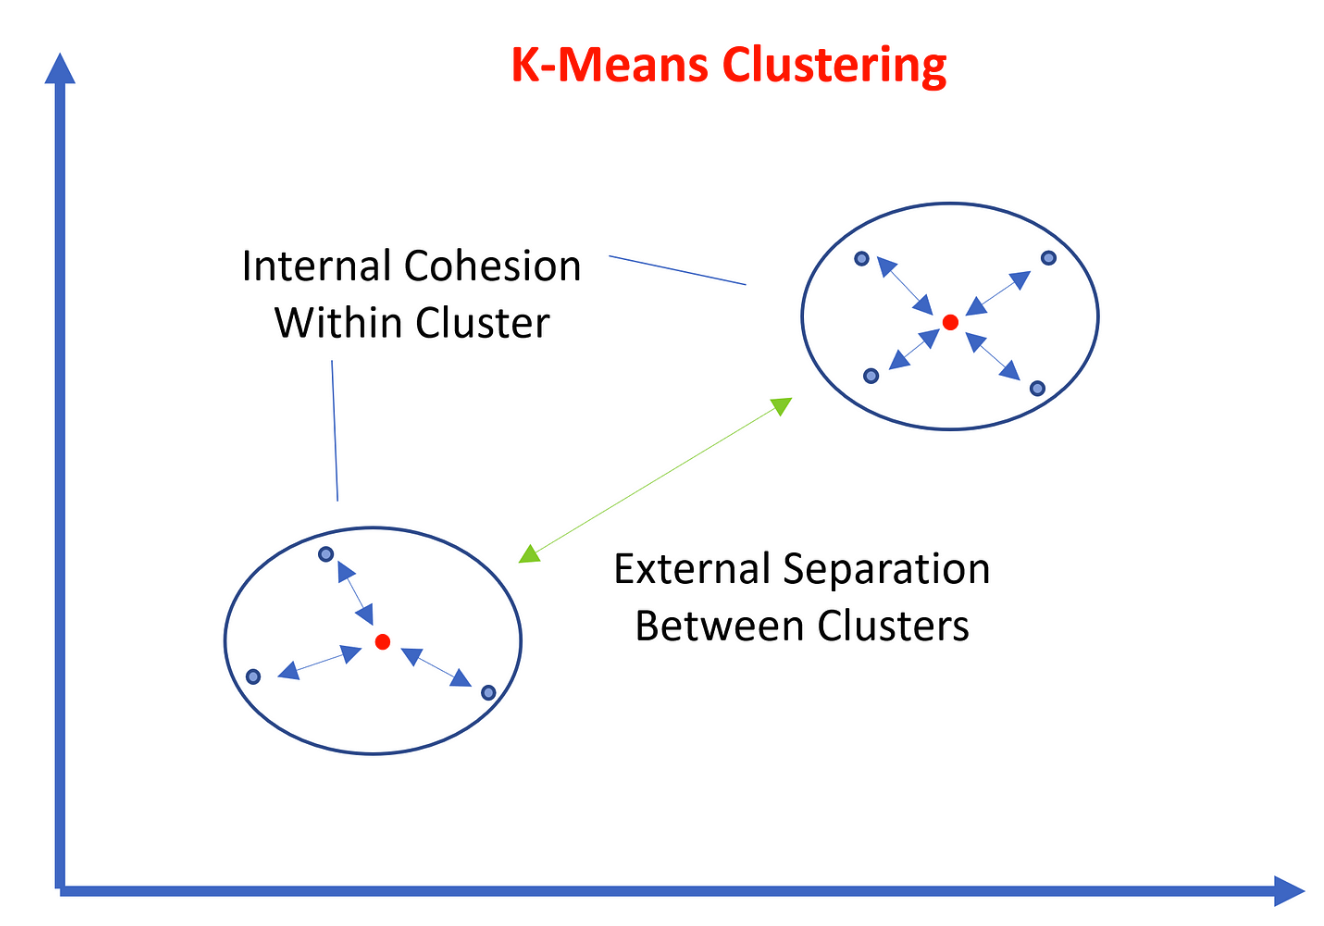
\epsfig{file=images/clustering_2,width=1.3\linewidth}}
  % \end{minipage}

% \begin{itemize}
%  \item 
% Data represented as a matrix $Y$ with dimensions $n\times m$ ($n$ could be species., $m$ could be sites) where
%   \begin{equation*} 
%       y_{ij} \in \{1,\ldots,q\} \hspace{25pt} i=1,\ldots,n \hspace{15pt} j=1,\ldots,m \hspace{15pt} q\;categories.
%   \end{equation*}
% \pause
%   \item \color{black}{For example, Spider data: }
%       \begin{itemize}
% 	\scriptsize
% 	\item $n=12$ species (rows)
% 	\item $m=28$ sites (columns).
% 	\item $q=4$ categories: Absence (0),\\ \hspace{2cm} Presences: (0,25\%] (1), (25,65\%] (2) and (65,100\%] (3)
% \pause
%       \end{itemize}
% \vspace*{-0.5in}
% \begin{minipage}{0.6\textwidth}{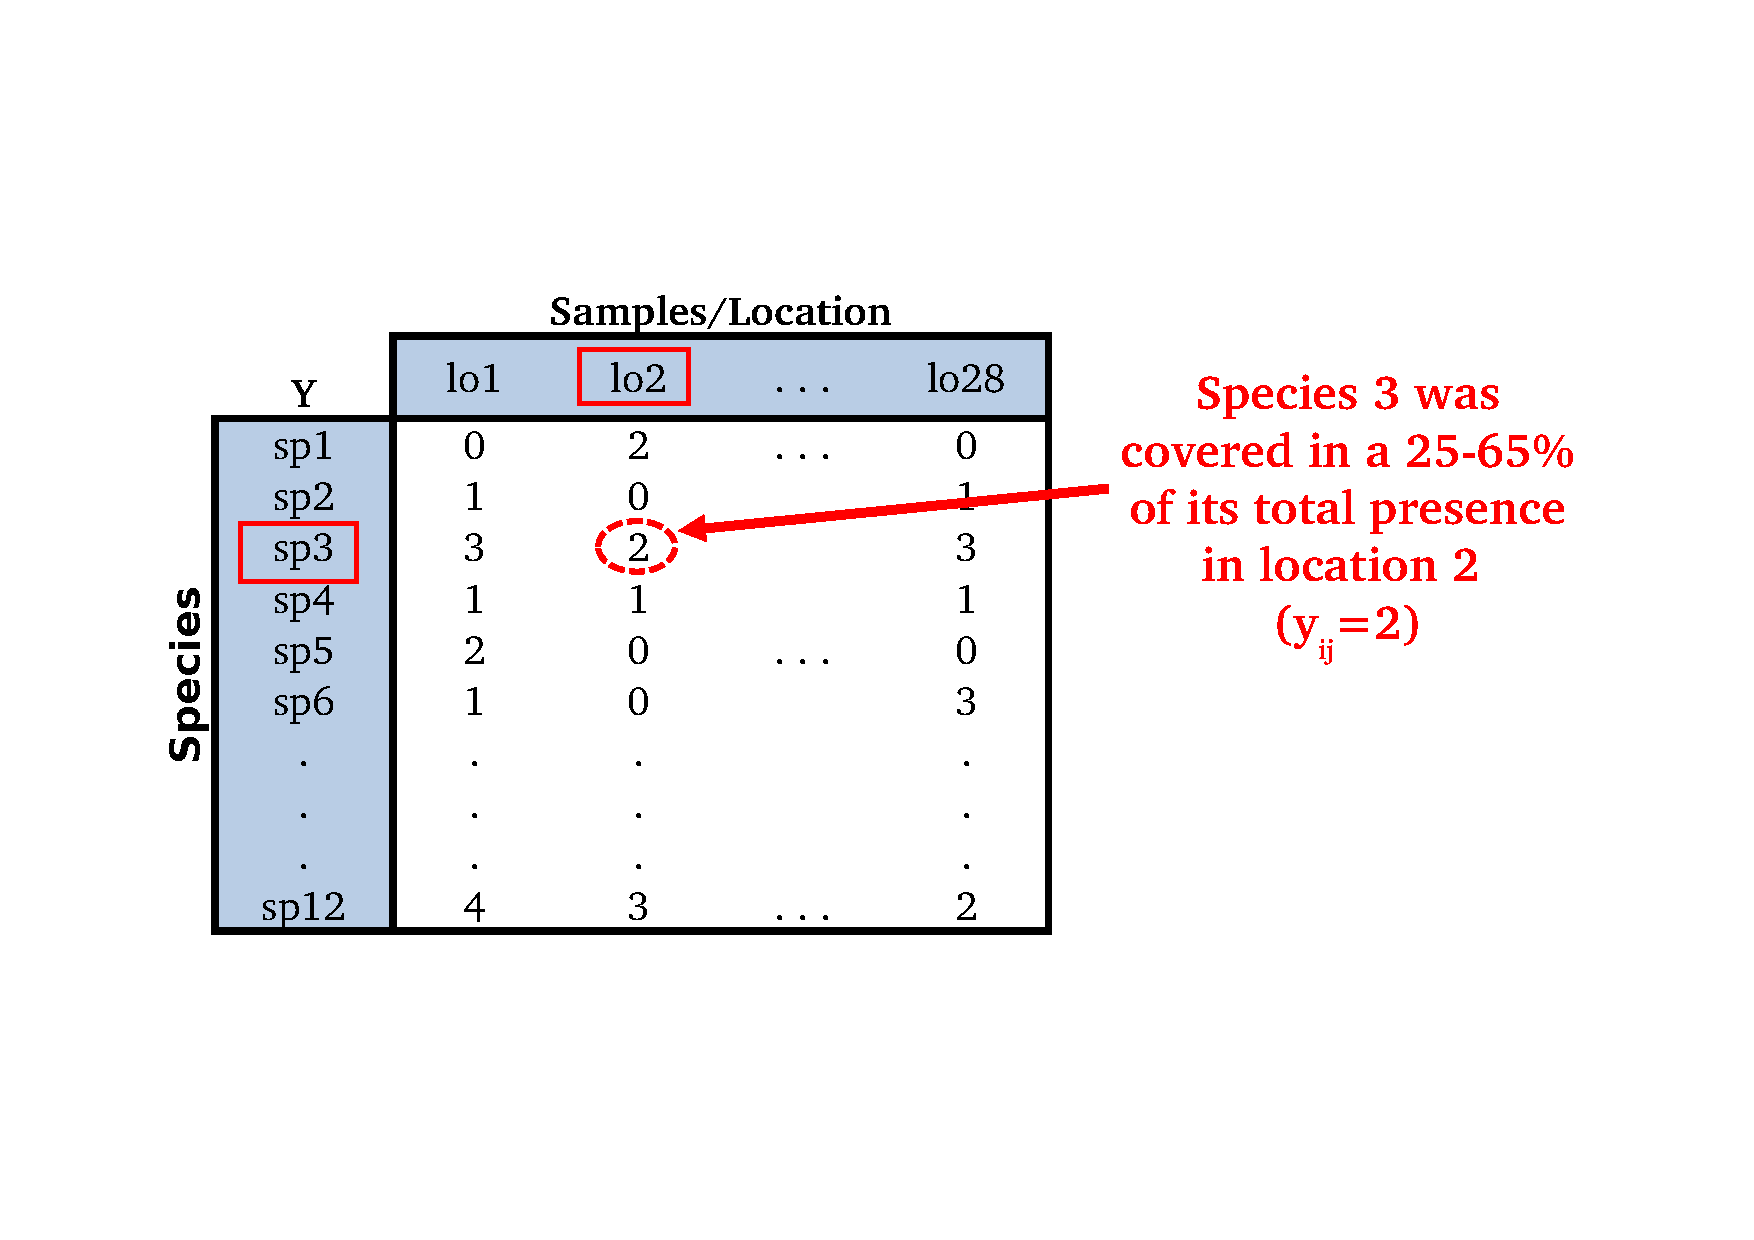
\epsfig{file=images/datamatrix_spider.pdf,width=1.3\linewidth}}\end{minipage}
% \end{itemize}

\end{frame}


%-----------------------------------------------------------------------------

\begin{frame}\frametitle{Finite Mixture Modeling}

  Unlike distance-based methods, statistical model-based clustering assumes that the data is generated from a mixture of finite distributions, where each component of the mixture represents a cluster. This approach tries to estimate the parameters of these distributions to optimize the fit between the model and the data.
  
  \begin{figure}
    \centering
    % If you continue using \epsfig
    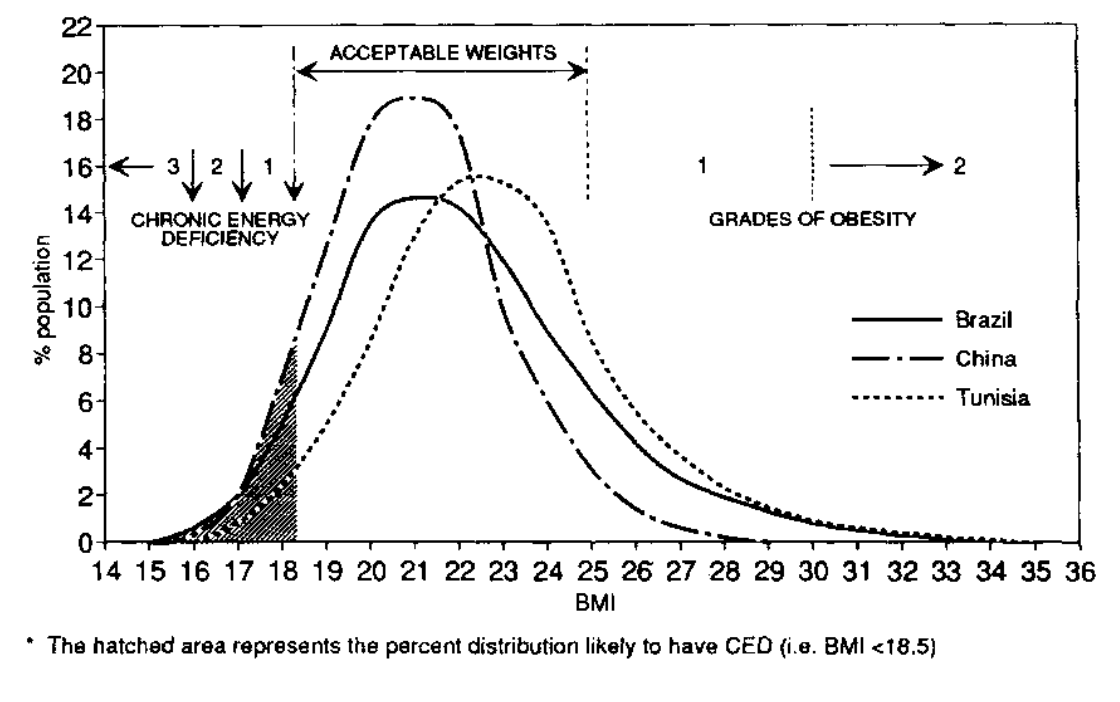
\epsfig{file=images/fmm_1,width=0.48\linewidth}
    % If you switch to \includegraphics from the graphicx package
    % 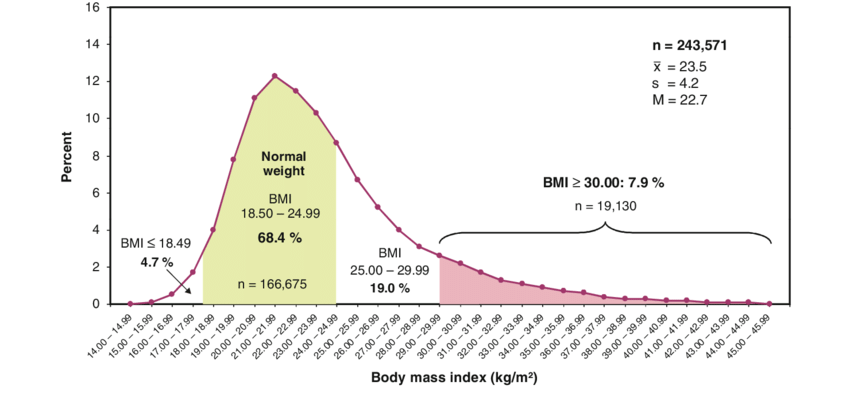
\includegraphics[width=0.6\linewidth]{images/bmi_2}
    \caption{mixture distribution between countries~\cite{shetty1994body}}
  \end{figure}
  
\end{frame}

%-----------------------------------------------------------------------------

\begin{frame}\frametitle{Bernoulli and Poisson distribution FMMS}

  \begin{figure}
    \centering
    \begin{minipage}{.48\linewidth}
      \centering
      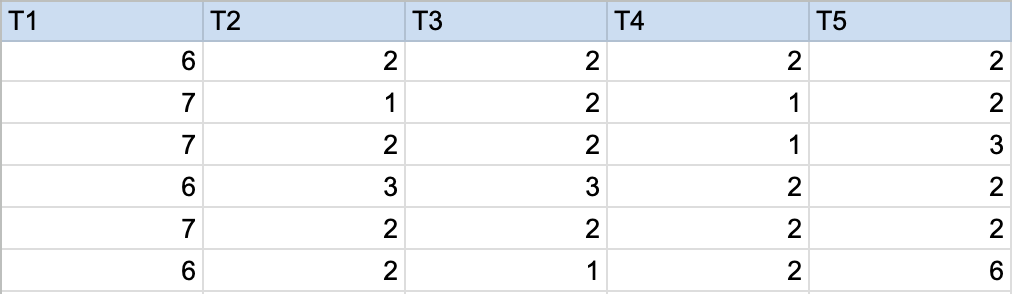
\epsfig{file=images/pmm,width=\linewidth}
      \caption{Apply Poisson  Distribution FMMs (for number of count)}
    \end{minipage}\hfill
    \begin{minipage}{.48\linewidth}
      \centering
      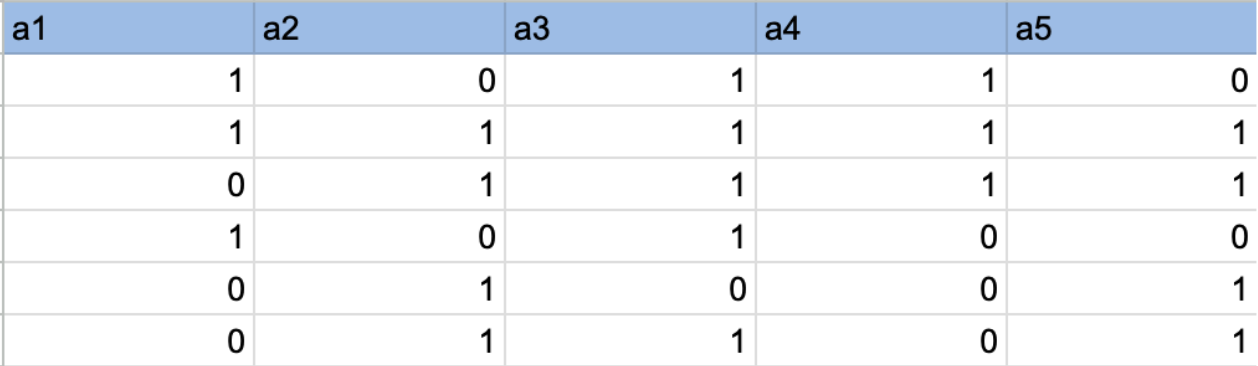
\epsfig{file=images/bmm,width=\linewidth}
      \caption{Apply Bernoulli Distribution FMMs}
    \end{minipage}
  \end{figure}
  
\end{frame}

%-----------------------------------------------------------------------------

\begin{frame}\frametitle{Methods: Finite Mixture Model}

  The Finite mixture model is defined as:
\begin{equation}
p(x_i|\mathbf{\Theta}) = \sum_{k=1}^{K} \pi_k f(x_i|\theta_k)
\end{equation}
% where:
% {\small
% \begin{itemize}
%     \item $p(x_i|\mathbf{\Theta})$ denotes the overall mixture model's density or mass function for observation $x_i$.
%     \item $K$ is the total number of component distributions in the mixture.
%     \item $\pi_k$ represents the mixing proportion of the $k$th component, satisfying $0 \leq \pi_k \leq 1$ and $\sum_{k=1}^{K} \pi_k = 1$.
%     \item $f(x_i|\theta_k)$ is the probability density function (pdf) or probability mass function (pmf) of the $k$th component distribution evaluated at $x_i$.
%     \item $\theta_k$ denotes the parameter vector of the $k$th component distribution.
%     \item $\mathbf{\Theta}$ symbolizes the complete set of parameters for the mixture model, including both the mixing proportions $\{\pi_1, \ldots, \pi_K\}$ and the parameters of the component distributions $\{\theta_1, \ldots, \theta_K\}$.
% \end{itemize}
% }

\begin{figure}
  \centering
  % If you continue using \epsfig
  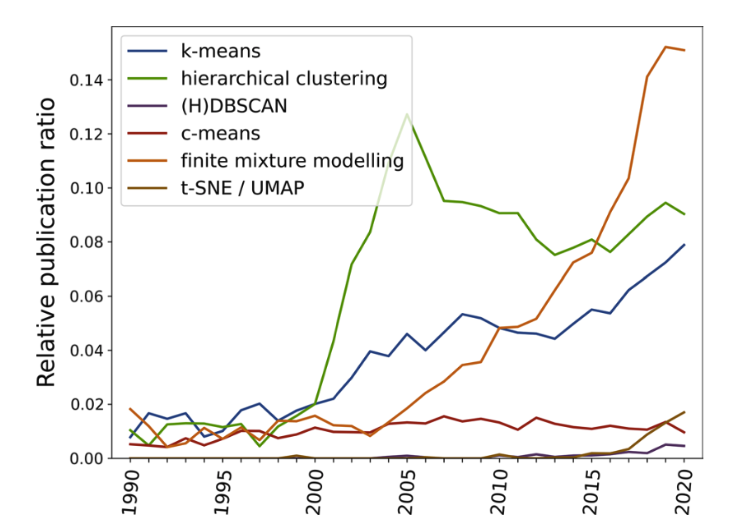
\epsfig{file=images/fmm_2,width=0.6\linewidth}
  % If you switch to \includegraphics from the graphicx package
  % 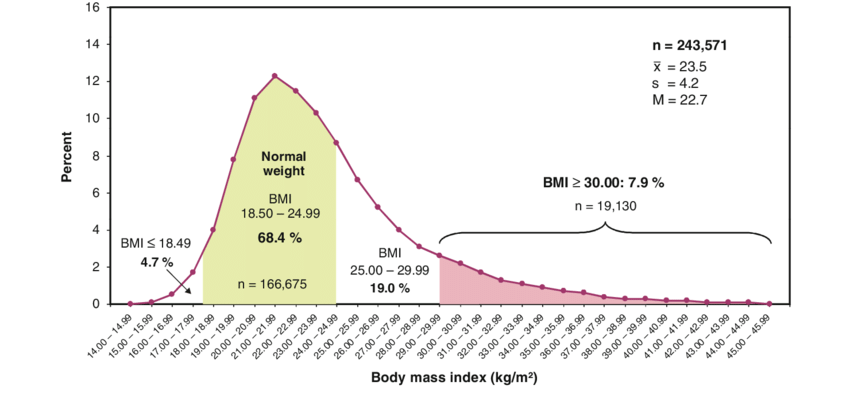
\includegraphics[width=0.6\linewidth]{images/bmi_2}
  \caption{FMMs publications index trend~\cite{fmmtrend}}
\end{figure}

\end{frame}

%-----------------------------------------------------------------------------

\begin{frame}\frametitle{Methods: Proportional Odds Model}

  Proportional Odds Model~\cite{mccullagh1980regression} Given an ordinal response variable $Y$ with $J$ ordered categories ($j=1, 2, \ldots, J$), 
  and a set of predictor variables represented by the vector $X$, the model expresses 
  the cumulative log odds of $Y$ being less than or equal to category $j$ as follows:
  
  \[
    \log\left(\frac{P(Y \leq j | X = x)}{P(Y > j | X = x)}\right) = \theta_j - \beta^T x
    \]

  where:
  {\small
    \begin{itemize}
        \item $P(Y \leq j | X = x)$ denotes the cumulative probability of $Y$ being in category $j$ or any category below $j$, given the predictors $X=x$.
        \item $\theta_j$ is the intercept for category $j$, and $\beta$ is a vector of coefficients for $X$.
        \item and $\beta$ is a vector of coefficients for $X$. $\beta^T x$ models the effect of the predictors on the log odds.
    \end{itemize}
  }
  
  
\end{frame}

%-----------------------------------------------------------------------------

\begin{frame}\frametitle{Methods: Ordered Stereotype Regression Model}

  Ordered Stereotype Regression Model~\cite{anderson1984regression}. 
  % Given an ordinal response variable $Y$ with categories ($j=1, 2, \ldots, J$), and a vector of independent variables $X$, 
  The probability of $Y$ falling into the $j$th category, given $X = x$, is denoted as $P(Y = j | X = x)$.

The logit for category $j$ is then:
\[
\log\left(\frac{P(Y = j | X = x)}{1 - P(Y = 1 | X = x)}\right) = \theta_j + \phi_j \beta^T x
\]
where:

{\small
    \begin{itemize}
        \item $\theta_j$ is the intercept for category $j$, and $\beta$ is a vector of coefficients for $X$.
        \item Stereotype model is unconstrained, $\phi$ add restricts to make it works for ordinal data. $1 = \phi_1 \geq \phi_2 \geq \ldots \geq \phi_k = 0.$ 
\end{itemize}
}

\end{frame}

%-----------------------------------------------------------------------------

\begin{frame}\frametitle{Methods: EM Algorithm}

  Finite Mixture model is implemented by E-M algorithm.
In E-step, update variables
each observation will be put into components (clusters) based on current distribution parameters
In M-step, update parameters
The parameters of each component will be update based on the observation adjustment
Repeat E-M step until converged (difference between parameter estimates below the threshold)


\begin{figure}
  \centering
  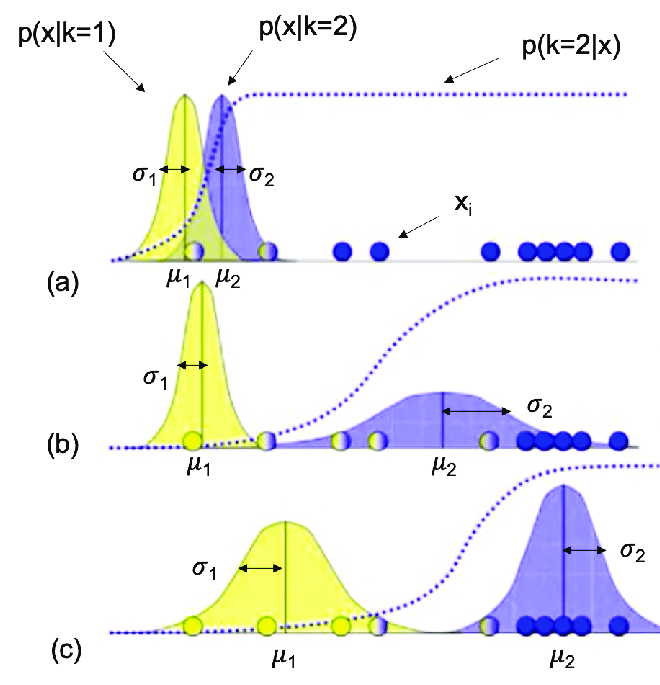
\epsfig{file=images/em,width=0.33\linewidth}
  \caption{E-M Algorithm~\cite{phdthesis}}
\end{figure}

\end{frame}

%-----------------------------------------------------------------------------

\begin{frame}\frametitle{Methods: Prediction Task}

  \begin{itemize}
    \item Prediction the cluster of new observation, based on the pre-trained FMMs Model
    \item Prediction will not update the parameter on each components (clusters)
    \item The benefit is prediction no need to repeat the E-M algorithm which is high cost. This approach is more effective and low cost. 
    
  \end{itemize}

\end{frame}

%-----------------------------------------------------------------------------

\begin{frame}\frametitle{Methods: Prediction Process}

  \begin{figure}
    \centering
    % If you continue using \epsfig
    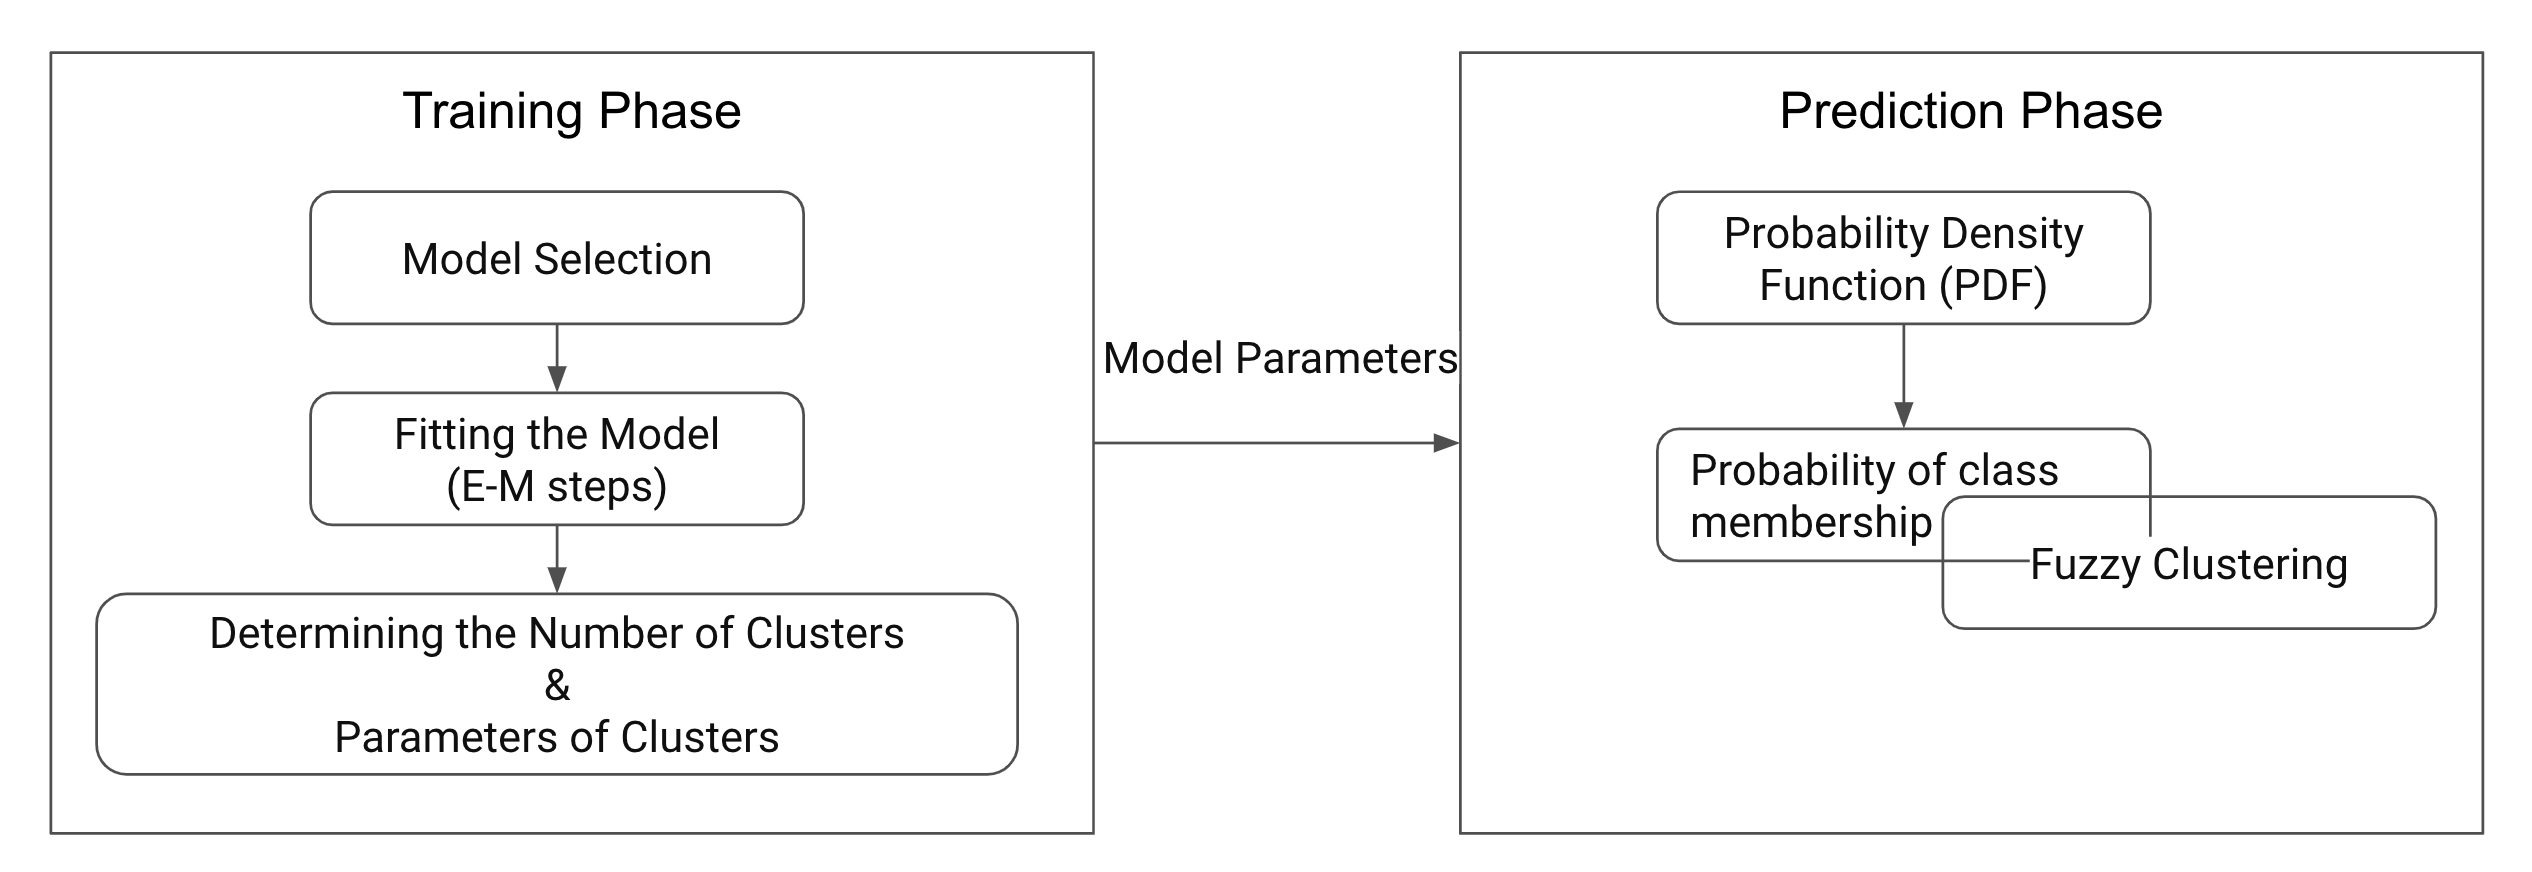
\epsfig{file=images/process,width=1.0\linewidth}
    % If you switch to \includegraphics from the graphicx package
    % 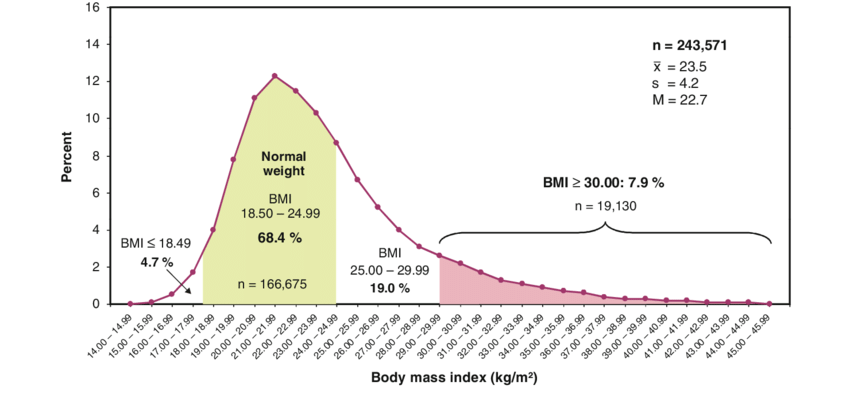
\includegraphics[width=0.6\linewidth]{images/bmi_2}
    \caption{new observation cluster prediction process}
  \end{figure}

\end{frame}

%-----------------------------------------------------------------------------

\begin{frame}\frametitle{Research Goals}

  \begin{enumerate}
    \item Analyze performance of the prediction task of different models for kind of distributions
    \item Analyze performance of the prediction task of models for different types of distributions
  \end{enumerate}

  \vspace{1em}
  \hspace{1em}\textbf{Notes}: This work will based on Real DataSet.


\end{frame}

% %--------------------------------------------------------
% \begin{frame}\frametitle{Background: Proportional odds model}

% Now, consider $Y$ has $c$ ordered categories.  For instance, let $c=3$ ( 1=''worse'', 2=''unchanged'', 3=''better'').

% \pause
% \begin{minipage}{0.5\textwidth}{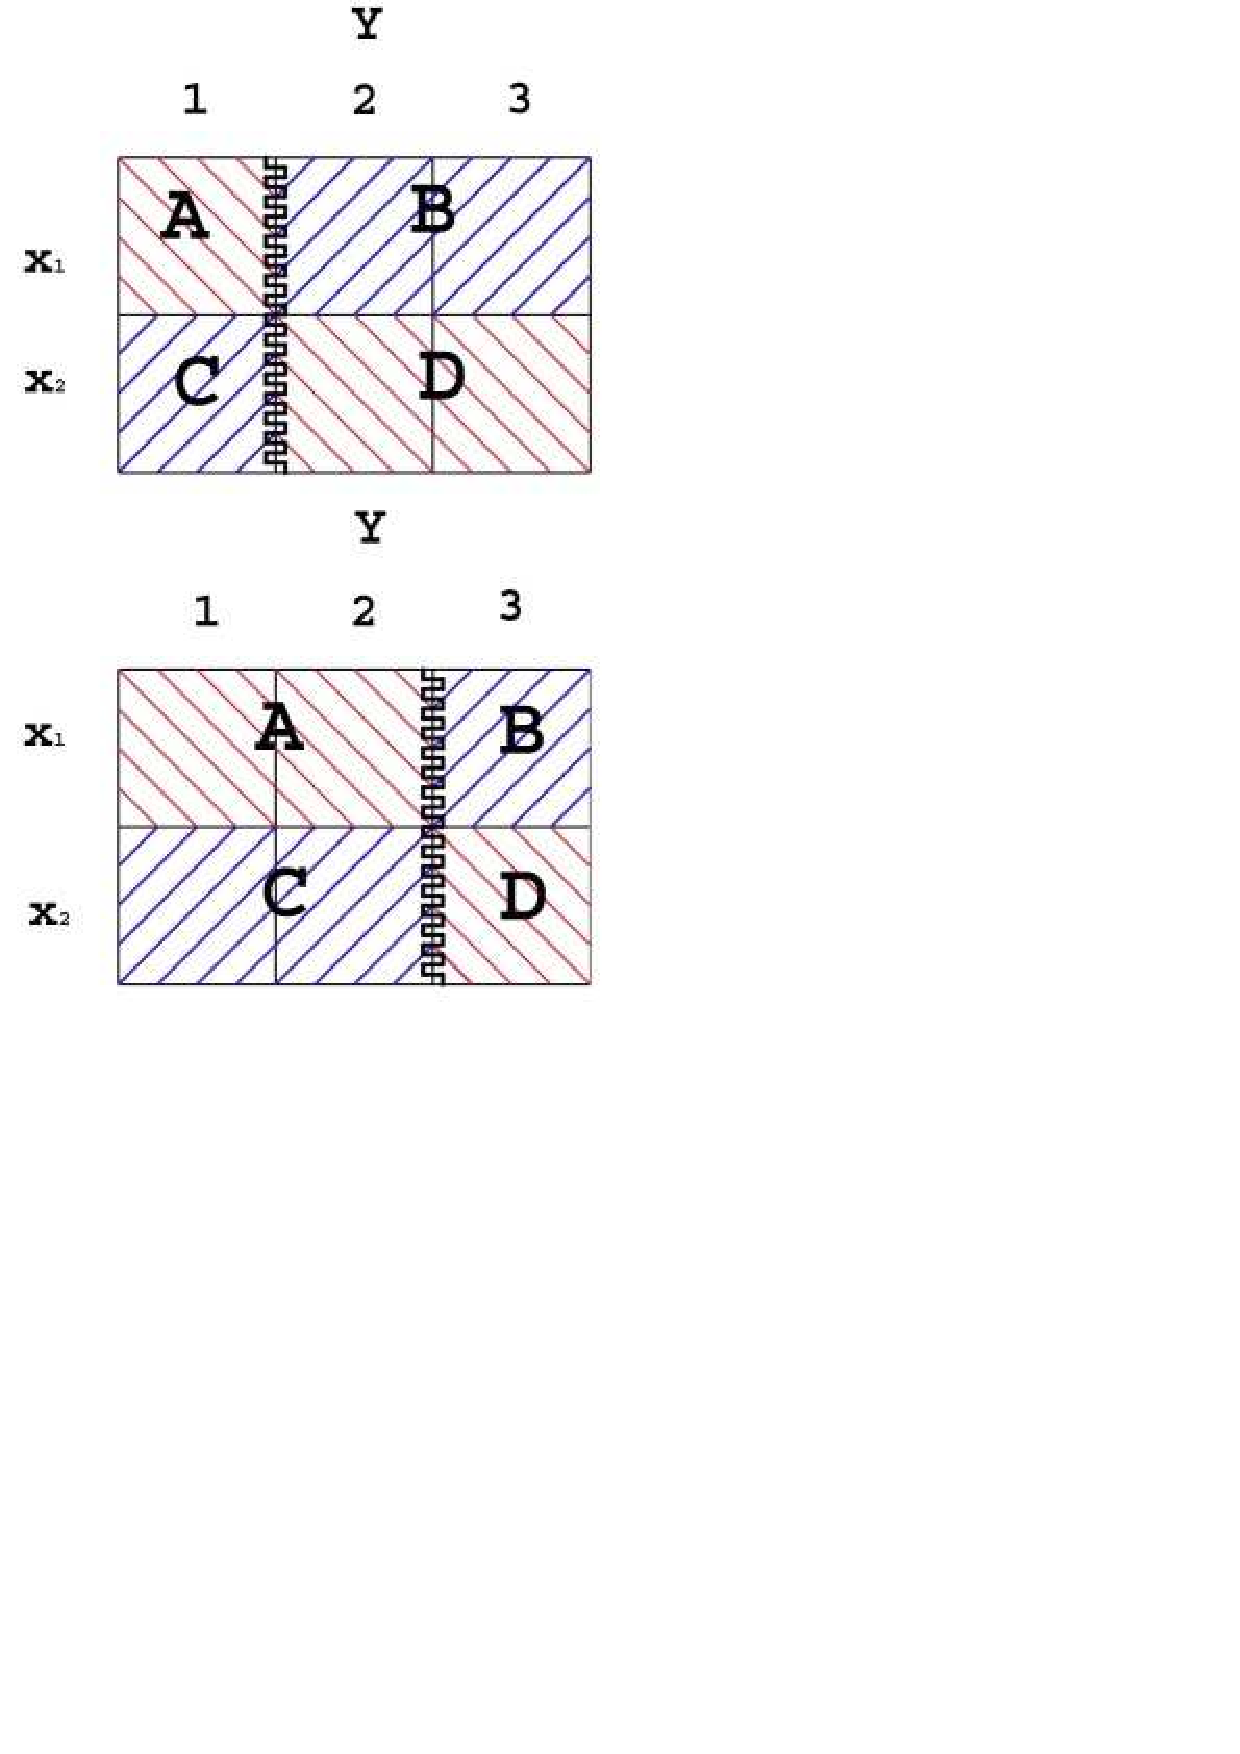
\epsfig{file=images/Pic2.pdf,width=1.3\linewidth}}\end{minipage}
% \begin{minipage}{0.45\textwidth}{\vspace{-1.5in}There are $c-1$  possible ways of collapsing a $c$-category response to a binary variable.\vspace{.2in}  \\  The proportional odds model implies that the odds
% ratios ($=\frac{A\times D}{B\times C}$) for describing effects of $X$ on the response variable are the same for each of these tables.
% }\end{minipage}
% \end{frame}

%--------------------------------------------------------
\begin{frame}\frametitle{Reference}
\bibliographystyle{plain}
\bibliography{reference}
\end{frame}

\end{document}
